\chapter{Architecture and Technologies}
\label{chap:architecture}

\section{Architecture and Data Flow}
\label{sec:architecture}
The following is the delivered architecture design of the system. The red numbers denote the flow of data
and are explained below:
\begin{figure}[H]
	\centering
	\begin{tikzpicture}
		\node(P) {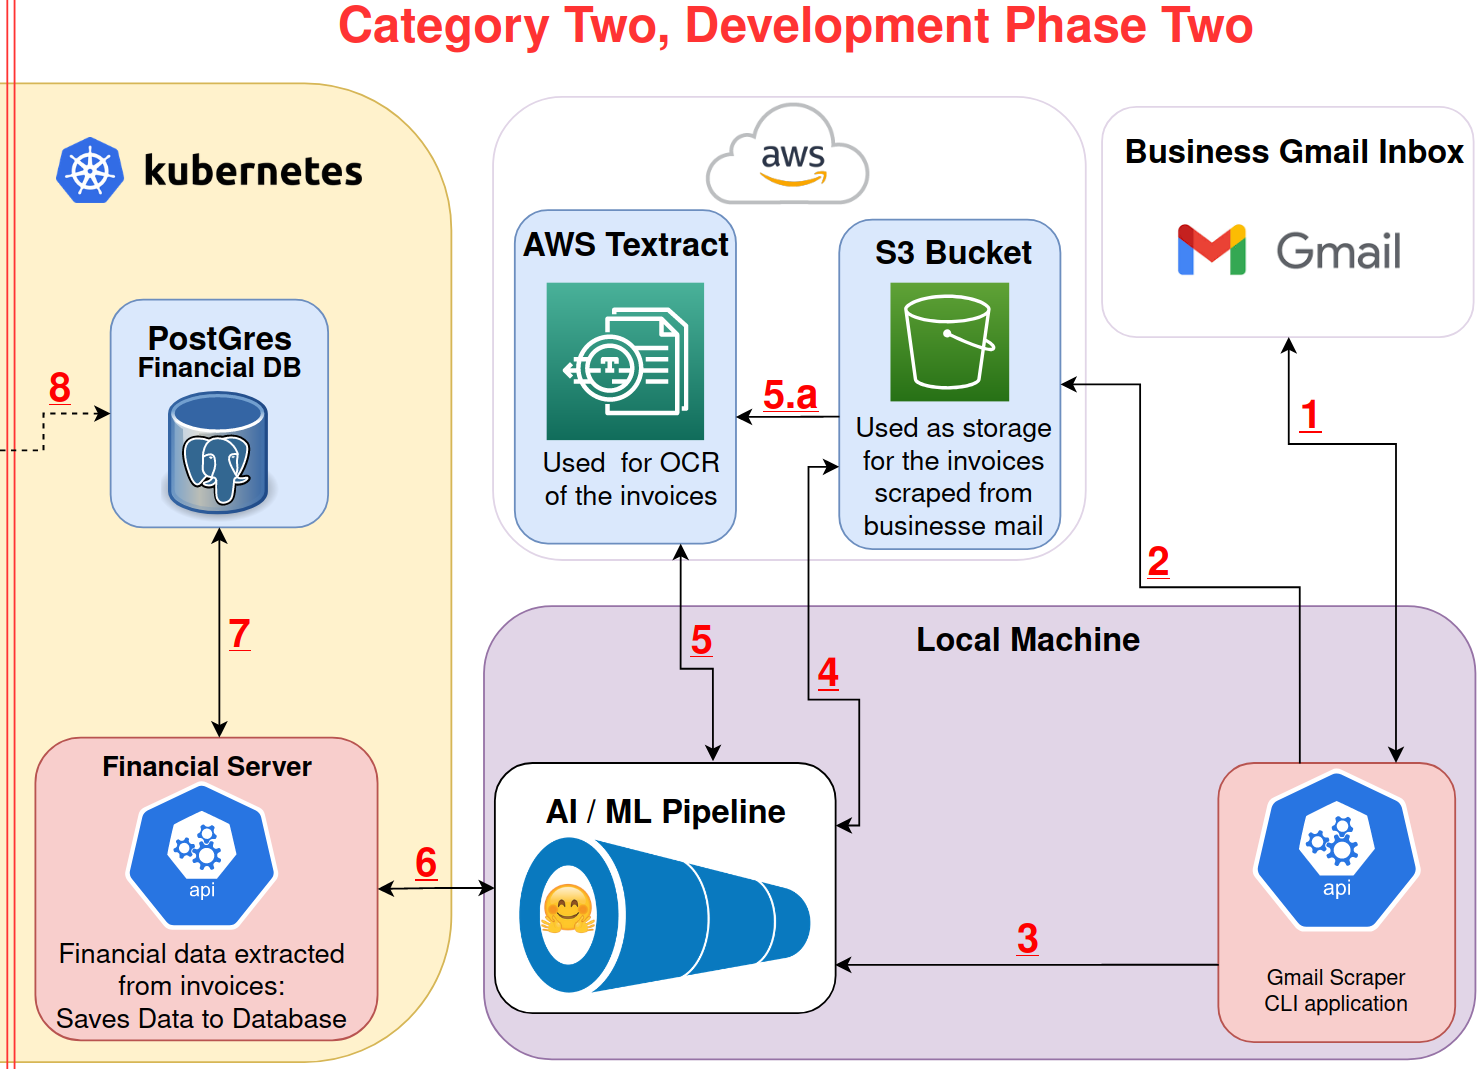
\includegraphics[width=1\linewidth]{figures/delivered_archi.png}};
		\tikzstyle{title} = [red]
		\node [title] at ($(P.north)+(0,0.2)$) {\Large{$(Semester~Two)$}};
	\end{tikzpicture}
	\caption{System Architecture}
	\label{fig:delivered_archi}
\end{figure}

\begin{enumerate} \label{enumerate:architecture}
	\item The Gmail Scraper CLI application scrapes the business' Gmail inbox for invoices.
	      It is currently configured to accept a scrape start date (until present time) and an
	      integer value for the number of invoices to scrape (this is for testing / demo purposes). \\
	      The CLI application is written in Python and uses the \code{imbox}~\autocite{rusevImboxPythonIMAP} package to scrape the
	      Gmail inbox.
	      \bigbreak
	      In a production environment, this would be altered slightly and deployed as a Lambda function
	      to periodically scrape the business' Gmail inbox.
	\item The Gmail Scraper saves invoices, which match the input criteria, to a secure S3 Bucket.
	\item The scraper then sends the invoice file name, location and Bucket name to the Machine Learning Pipeline (ML Pipeline),
	      which is deployed behind a Flask server, from here on it will be referred to as the \emph{\textbf{Inference Server}}.
	\item The Inference Server pulls the desired invoice locally.
	\item The Inference Server then requests Optical Character Recognition (OCR) data for the desired invoice via an AWS Textract API call.
	      This call tells Textract the location of the invoice in the S3 Bucket and the desired region.
	      \begin{enumerate}
		      \item AWS Textract obtains the invoice from the S3 Bucket and performs OCR on the invoice.
	      \end{enumerate}
	      When it finishes, the OCR data is sent to the Inference Server.
	\item The Inference Server then prepares the OCR data for inference in a pre-process step, once this step is complete the model
	      performs the inference.\\ The results from the inference are returned, and the data then goes through a final post-process step.
	      Once the inference and post-processing are complete, and the data is in the required format, the Inference Server sends the data
	      to the Financial Server.
	\item The Financial Server is another Flask server written in Python. The server is a running service located in the Kubernetes cluster.
	      The Financial Server utilizes the SQLAlchemey~\autocite{SQLAlchemyDatabaseToolkit} \emph{Object Relational Mapper (ORM)} as a
	      \emph{translational} layer to communicate with the Postgresql database, also deployed in the Kubernetes cluster.
	      The Financial Server saves the data to the Financials DB.
	\item The dotted line depicts the interaction between the Kafka consumer, obtaining and saving transactional data (not operational) to the
	      Financials database.
\end{enumerate}
\subsection{The Pivot, Explained}
\label{sec:pivot}
As can be seen by comparing the proposed architecture, \Cref{fig:sys_archi}, and the delivered architecture, \Cref{fig:delivered_archi},
the system architecture has been altered. The shift may look significant, but the components are fundamentally the same. As the deployment
of a full Kubernetes environment was prohibitively expensive, the system was deployed in a Minikube cluster. This actually
increased the complexity as components to link services running locally to services running in the Minikube cluster needed to be created. \\
The change in architecture is due to the following reasons:
\begin{itemize}
	\item As mentioned, Minikube is used as the development version of Kubernetes. In essence, it is a single node Kubernetes
	      cluster\footnote{For more information see section 2.2 \emph{Technologies Used} of the first report}.
	      The initial architecture, as per \Cref{fig:sys_archi}, is designed to incorporate the Inference Server into the
	      Kubernetes cluster. Whilst this is still possible, as the Inference Server is containerised and \emph{Kuberentes-ready},
	      Minikube does not allow external calls from inside the Kubernetes environment. This seems like a drastic limitation and was
	      not known before the choice of Minikube as the development Kubernetes tool. Minikube will allow endpoints exposed in the
	      cluster to be accessed from outside the cluster but only from the localhost system upon which Minikube is installed.
	\item Numerous, unsuccessful attempts were made to try and circumvent this limitation of Minikube including:
	      \begin{itemize}
		      \item Configuration of a Kubernetes Ingress resource in the cluster.
		      \item The use of Ngrok on the local machine to expose the Inference Server's endpoint to the internet.
		      \item The deployment of an Ngrok pod in the cluster to expose the Inference Server's endpoint to the internet.
	      \end{itemize}
	      The technical implementations of the above are further detailed in the \Cref{sec:challenges} section.
	\item The deployment of the Gmail Scraper application locally was primarily done to facilitate the demo and to aid in development. The
	      deployment of the Gmail Scraper to AWS Lambda can be achieved with a minor refactor.
\end{itemize}
As one can now visualise the data flow throughout the system components, the next step is a deeper dive into the technologies considered
for use in the system along with explanation of the chosen technologies and their implementation.
\section{Technologies Considered for the Inference Server - AI / ML Pipeline Structure}
\label{sec:technologies}
The Inference Server consists of the Artificial Intelligence  (AI) / Machine Learning (ML) pipeline, which is deployed behind a Flask server.
Whilst the implementation of a Flask server is trivial, the AI / ML pipeline was the most challenging component of the entire system. But also
the most interesting.\\
Other sections of this project had a large quantity of `known unknowns', this section has had a huge amount of `unknown unknowns'.
To extract desired key information from an invoice, the document must first go
through a series of steps where each step's input is dependent on the previous step's output. This is why the term used is in industry is
`pipeline'. The approach to tackling this problem must first be outlined:

\subsection{Three-Step Process}
To solve the KIE from an invoice problem, this is the three-stage process that will be used:
\begin{enumerate}
	\item \textbf{Text Localisation}: For this step a model is used to identify the location of text in the invoice. The text is
	      wrapped in bounding boxes. As per \Cref{fig:bounding_box_partial}:
	      \begin{figure}[H]
		      \centering
		      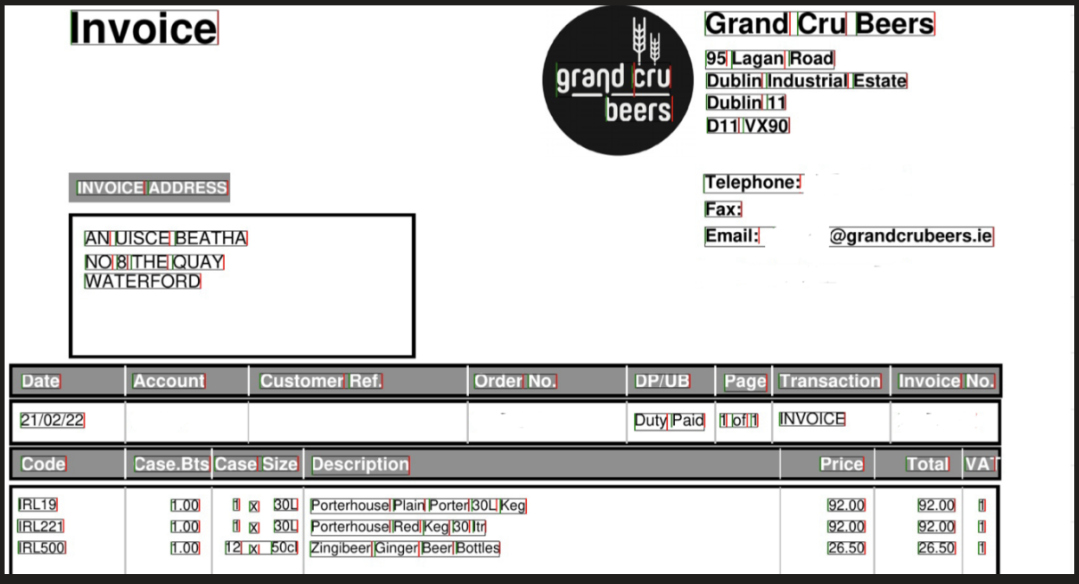
\includegraphics[width=0.8\linewidth]{figures/bounding_box_partial.png}
		      \caption[Bounding Box Example]{An example of the bounding boxes. The locations of each word / text are detected, and a bounding box is created
			      around each piece of text. For clarity, this example has the bounding boxes drawn on. The start of each word starts with a green line and finishes with red.\\
			      \textbf{Note:} Some of the text has been removed as these are real documents which contain sensitive data.}
		      \label{fig:bounding_box_partial}
	      \end{figure}
	      This step is not the most difficult and there exist many open-source models that can achieve this with relatively good performance metrics.
	\item \textbf{Optical Character Recognition (OCR)}: For this step the bounding boxes obtained from the initial step are used by a model to extract
	      the text from the image. The text is returned in the form of a key value pair, where the key is the text and the value is the bounding box or vice versa.\\
	      This step is also not the most difficult and models exist such as Tesseract and OpenCV that can achieve this, also with relatively decent performance
	      metrics. As previously alluded to, the problem lies with the pipeline effect.
	      \bigbreak
	      If the Text Localisation stage is not successful or optimal then there is no way any subsequent step can
	      return the desired information. For example, if the Text Localisation step is 90\% accurate, The best result that can be returned from the OCR step and
	      subsequent steps is, theoretically, 90\%.\\
	      Although just `theoretically' as in practice no ML step is ever 100\% accurate, therefore, each subsequent step will bring with
	      them their \emph{`price'}, a reduction in performance.\\
	      This is why it is crucial that all steps are as accurate as possible as the third and final step is, by an order of magnitude, more difficult
	      than the previous two.
	\item \textbf{Key Information Extraction (KIE)}: This is the fascinating step. There are no real open source models, like Tesseract for OCR, of any
	      real merit for KIE. This may be because of a lack of research in general along with the variance in source data.
	      The lack of any kind of standard or structure for receipts, but in particular for invoices makes this task all the more difficult.
	      The variance in data makes it very difficult to obtain a model that is generalized (can work on all / different forms of data).\\
	      A number of different approaches / model architectures can be used to try and accomplish this step.\\
\end{enumerate}
\subsection{Visually-rich Document Understanding Competition - SROIE}
From the three stage process as outlined above, the Text Localisation and the OCR steps have both open-source and very good proprietary models.
Not to say that they are trivial, as they most certainly are not, but the main area of interest is the KIE step.\\
In general, the area of visually rich document / semi-structured document understanding is not considered a solved problem in the discipline of
computer science. To the extent that organizations exist which run competitions to try and further this field. The largest of which
is a competition that was started in 2019 by a collaboration of universities from across the globe known as the \emph{Scanned Receipts OCR
	and Information Extraction (SROIE)} as part of the larger set of challenges in the area of computer vision, the \emph{Robust Reading Competition}
~\autocite{OverviewICDAR2019}. This is driven by the Computer Vision Center~\autocite{ComputerVisionCenter}, a specialised research campus
in the Universitat Autonoma de Barcelona (The Autonomous University of Barcelona). Along with a host of other universities from Shanghai to
Aston to Nanyang, amongst others.
\bigbreak
The organisers for this competition created one of the first publically available and largest datasets
(of receipts) for use in this competition, known as the SROIE dataset. The competition is still ongoing, there is a leader board and there are still entries being added periodically.
The following is an example of the SROIE dataset:
\begin{figure}[H]
	\centering
	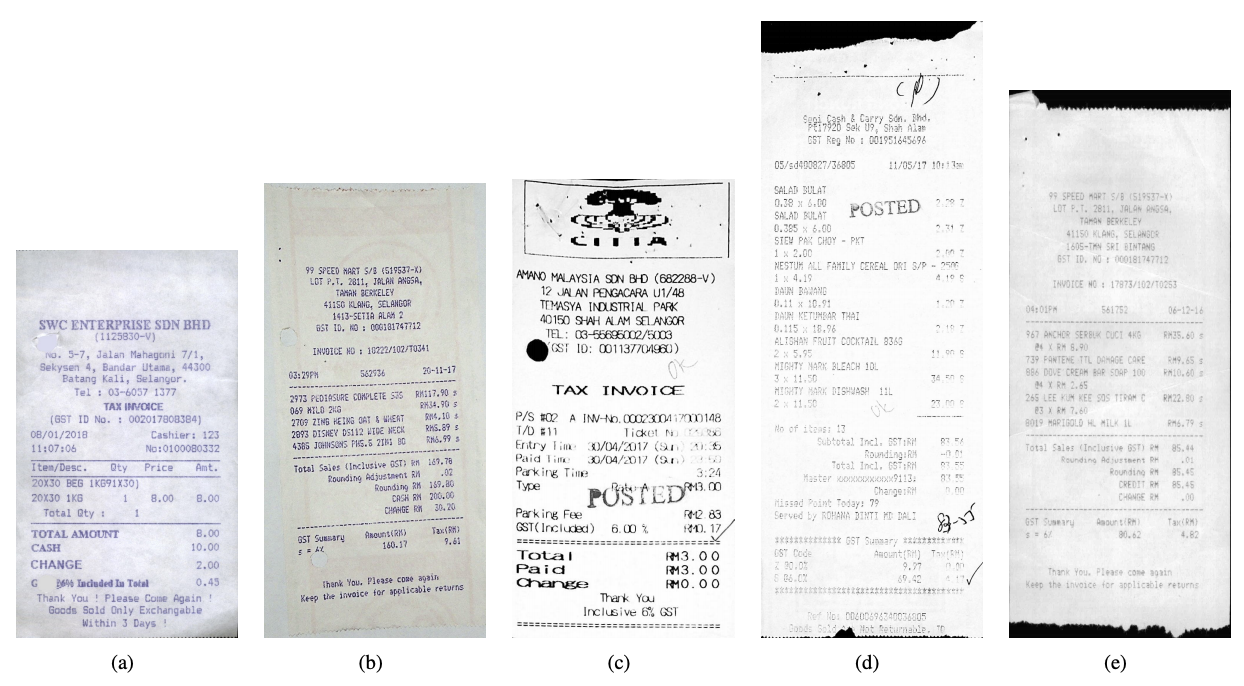
\includegraphics[width=1\textwidth]{figures/sroie_example.png}
	\caption{SROIE Dataset Example}
	\label{fig:sroie_dataset_example}
\end{figure}
The SROIE competition was, initially, the main focus of research for this project and was an invaluable source for gaining a look into the cutting
edge research carried out on visually rich document understanding~\autocite{MethodStrucTexTTask}. The papers also reveal the different approaches taken by
the participating teams.
\bigbreak
The SROIE website contains links to some open-source code repos for the entries. It was the perfect place to start research and to get a better
understanding of the problem space.
\begin{figure}[H]
	\centering
	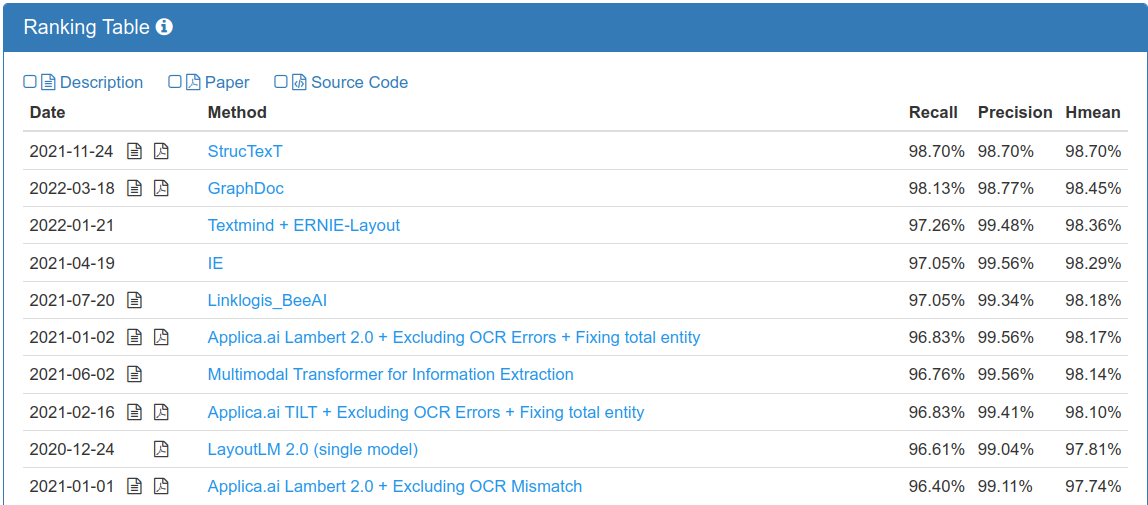
\includegraphics[width=1\linewidth]{figures/SROIE_results.png}
	\caption[SROIE Results (KIE)]{The current results of the SROIE competition in the KIE task.\\
		\textbf{Note:} An interesting observation is that the overwhelming majority of the top end of the leaderboard are all using some variation of a model
		based on the \emph{transformer} architecture.}
	\label{fig:SROIE_results}
\end{figure}
The methods used by different teams vary greatly as can be seen in the ranking graph~\autocite{ResultsICDAR2019a} by the large variation in both models
used and scores achieved.\\
Some very large and innovative tech companies have entries in the competition including Baidu, Microsoft, Tencent and Samsung to name but a few.
\bigbreak
It must be noted that the dataset differs substantially from the use case for this project. No publically available dataset (of invoices) was available for
this project, so one was created from the authors personal business.
\bigbreak
A further point of interest is that the SROIE competition requires only four fields, to be extracted. As such most projects limited their
tags (the tagged field i.e. \code{total\_amount} for receipt total) to four fields - company, date, address, and total. For comparison, this project
ended up with over 20 fields in order to extract the desired information.
\bigbreak
Whilst format of receipts differs, the variance is not that great. Most receipts have a similar structure. The same can not be said about
invoices. For invoices, the structure is much more varied as to are the borders / boxes / white space which separate the values.
\subsection{SROIE Models}
Whilst these differences posed challenges to completing this project, it was none-the-less decided to start trying to implement some of the open-source models
from the competition. The initial attempts proved to be extremely time-consuming and joyless. The text localisation models were attempted first. From
5 models attempted, only one was successful in deployment.
\bigbreak
The attempts at running the OCR models proved a little more successful with two of four being successfully deployed. No KIE models could be successfully
deployed from the competition.\\
There were many factors which added to the many unsuccessful attempts:
\begin{itemize}
	\item The models used varied greatly in the dependencies needed to run and the versions of the different packages used. There is a considerable
	      difference in running a model on PyTorch and Tensorflow / Keras.
	\item An initial lack of implementation / deployment experience or initial working knowledge of Python and its dependencies structure
	      increased the difficulty level.
	\item Another obstacle was that most of the repos contain comments and explanations of the code in Mandarin. This was an interesting observation.
	      The vast majority of entries were from China\footnote{Considering the driving force is a European University and part of the funding for the competition came
		      from the EU, the overwhelming majority of the entries being from China was a surprise. That said, most of the entries in the top 10s in all three tasks
		      were Chinese. It is clear the country focuses its universities in this area.}.
	\item Once the initial obstacles and challenges were cleared. The biggest limiting factor in the reproduction of the model deployment became apparent.
	      The models used by teams were trained with machines with more than the GPU memory on the development machine for this report. At 4gb of GPU memory, the
	      hardware limitations were proving to be a problem. Even with pretrained models and weights available from one or two of the repos.
\end{itemize}
Only a single Text Localisation model could be successfully run on the development machine and the other successful attempts came from running models
on AWS ec2 instances optimised for GPU memory. Although this too came with limitations as the instances with GPU access are expensive and there are no
free tier options for the hardware needed. At this point a different approach was needed.
\bigbreak
Instead of merely trying to implement the open source models as per the repo, it was decided to look at some of the top performing models and try to implement
a solution from scratch. It was during this research that the LayoutLMv2~\autocite{xuLayoutLMv2MultimodalPretraining2022} model was discovered. This is a newly open
sourced model, released toward the tail end of 2021 by Microsoft Azure AI~\autocite{ArtificialIntelligenceResearch}, and it showed some great promise both in
terms of performance and in terms of model size, due to the model utilizing \emph{transfer learning} (more details to follow). This model designed especially
for visually-rich documents.\\
Implementations of the original LayoutLM model were consistently near the top of the leaderboard for the KIE in the SROIE competition. As to were
other models like BERT~ber\autocite{BERT} and other variations of BERT like LamBERT~\autocite{LAMBERT2022} and RoBERTa~\autocite{RoBERTa}. These models all share something in common, they are all built on the same
\emph{Transformers} architecture.
% so here talk about transformers architecture and all the shite i outlined to kieran
\bigbreak
\section{Transformers and the LayoutLMv2 Architecture}
As LayoutLMv2 is a \emph{Transformers} based model, this section will outline the main concepts underpinning the transformers architecture with a particular focus
on the differences and additions that make up the LayoutLMv2 model\footnote{This section is by necessity quite technical, but there are a number of great
	resources to introduce this topic in more detail than what is summarized here and can be found in this excellent
	series of articles~\autocite{doshiTransformersExplainedVisually2021}.
	Some other great articles on the topic, here~\autocite{munozAttentionAllYou2021}, here~\autocite{cristinaTransformerModel2021}
	and here~\autocite{alammarIllustratedTransformer}.}.
% But first, a little bit of background as to the developments which have led to t
\bigbreak
The Transformers architecture has revolutionized the area of Natural Language Processing (NLP) since its architecture was proposed in
the excellent paper \emph{Attention Is All You Need}~\autocite{vaswaniAttentionAllYou} developed by Vaswani et al. at Google in 2017.
\bigbreak
This architecture is used as the backbone and therefore has given rise to a number of very famous and powerful models such as the
aforementioned BERT~\autocite{BERT} and OpenAI's GPT series of models, the latest of which is the GPT-3 model~\autocite{GPT3PowersNext2021}.
The GPT-3 model has a massive variety of use cases such as English to other language translation (French, Spanish and Japanese are some of the
languages supported), Python code to Natural Language, as per \Cref{code:GPT3_NL_translation} and many others.
A more comprehensive list can be found here~\autocite{GPT3PowersNext2021}:
\begin{lstlisting}[language=python, label={code:GPT3_NL_translation}, caption={GPT-3 Python code for human language translation as per~\autocite{OpenAIAPI}}]
def remove_common_prefix(x, prefix, ws_prefix): 
    x["completion"] = x["completion"].str[len(prefix) :] 
    if ws_prefix: 
        # keep the single whitespace as prefix 
        x["completion"] = " " + x["completion"] 
return x 

# Output generated by GPT-3:
# The code above is a function that takes a dataframe and a prefix as input and returns a dataframe with the prefix removed from the completion column.
\end{lstlisting}
\bigbreak
\textbf{Note}: not all of the output is as coherent and accurate as the chosen example, although a sub-product of GPT-3 can be found powering tools
such as GitHub Co-Pilot which is a tool to aid developers by making suggestions for code completion based on the context of the code already written or
by the comments written in the code which Co-Pilot can then use to suggest code completion and / or code generation with very decent results in real time.\\
This is just a single example of the type of applications for these type of models.
\bigbreak
Before Vaswani's paper, the state-of-the-art models for NLP were Recurrent Neural Networks (RNNs) and Convolutional Neural Networks (CNNs) which implemented an
\emph{encoder} and a \emph{decoder}. These types are known as sequence to sequence models (seq2seq) as a sequence is used as the input and output.
\bigbreak
For example, Machine Translation (MT) is a seq2seq model where the input is a string of words and the output is a translation in another language for the
input string. This was the initial use case for the Transformers architecture, although English to French and French to German were the chosen
languages\footnote{The Greek translation is pronounced `Yasu Cosme'}.
\begin{figure}[H]
	\centering
	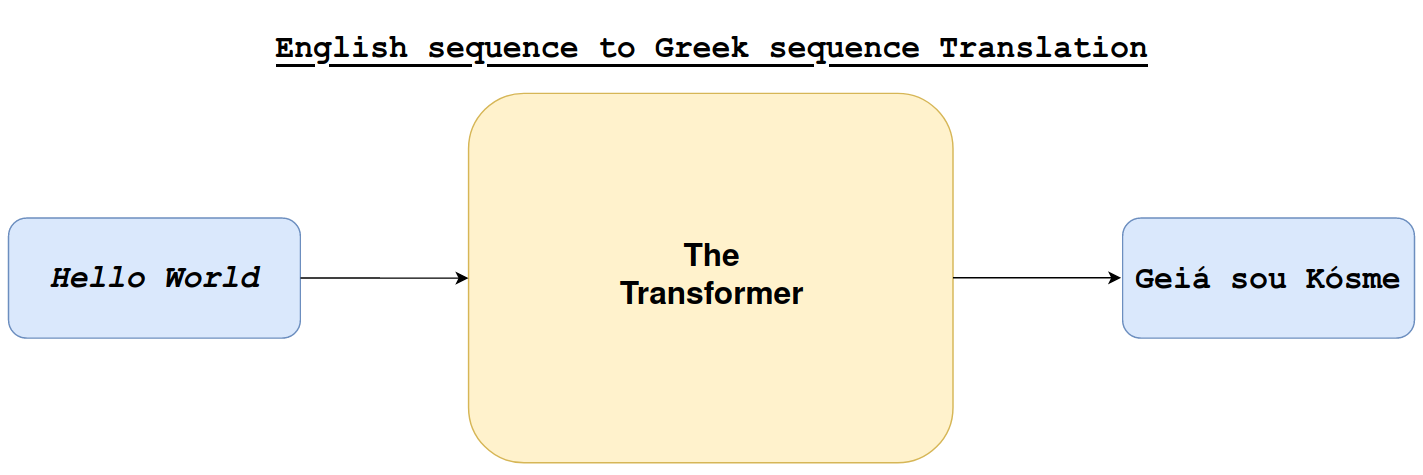
\includegraphics[width=0.8\linewidth]{figures/basic_transformer.png}
	\label{fig:basic_transformer}
	\caption{Basic Transformer Sequence To Sequence example}
\end{figure}
\subsection{Encoder and Decoder High Level Overview}
Peeking under the hood, we can see that the encoder and decoder are responsible for the translation. The original paper proposed a stack of
six encoders and similarly a matching set stack of six decoders, although these numbers can be altered.
\begin{figure}[H]
	\centering
	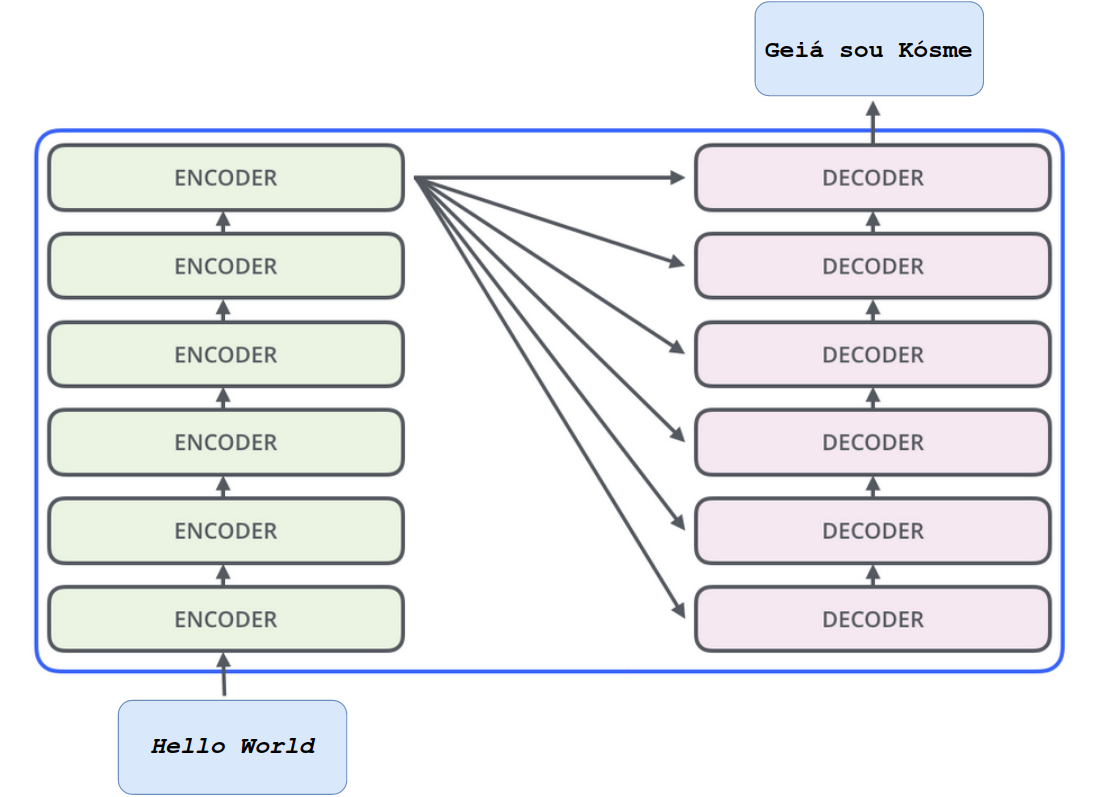
\includegraphics[width=0.9\linewidth]{figures/transformer_stacked_encoder_decoder.png}
	\label{fig:transformer_stacked_encoder_decoder}
	\caption{Transformer Stacked Encoder and Decoder example, sourced from here~\autocite{alammarIllustratedTransformer}}
\end{figure}
The encoder itself are identical in structure, but they have their own weights associated to them. At first these are set at random, but they are
altered through the back-propagation of the training phase (details to follow).
\begin{figure}[H]
	\centering
	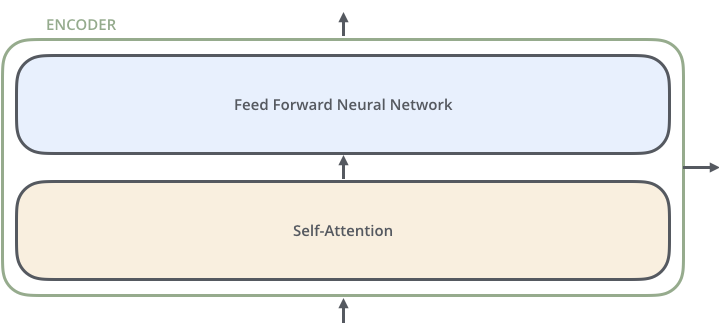
\includegraphics[width=0.8\linewidth]{figures/encoder_architecture.png}
	\caption{Transformer Encoder architecture example, sourced from here~\autocite{alammarIllustratedTransformer}}
	\label{fig:transformer_encoder}
\end{figure}
The Self-Attention layer will be described in more detail shortly but for now lets look at the decoder architecture:
\begin{figure}[H]
	\centering
	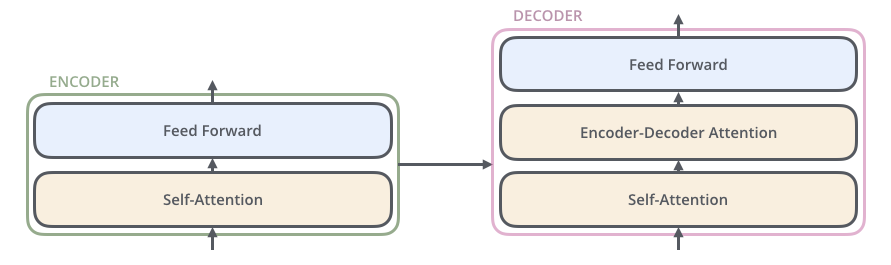
\includegraphics[width=1\linewidth]{figures/decoder_archi_1.png}
	\caption{Transformer Decoder architecture example, sourced from here~\autocite{alammarIllustratedTransformer}}
	\label{fig:transformer_decoder}
\end{figure}
As is observed the decoder is almost identical to the encoder save for an added \code{Encoder-Decoder} layer. This layer
\emph{helps} the decoder to `focus' on the relevant part of the input sequence.
Now that we have a very high level idea of the main components of the Transformers architecture, we can look at the actual architecture of
the original Transformers model.
\subsection{Original Transformers Architecture}
\begin{figure}[H]
	\centering
	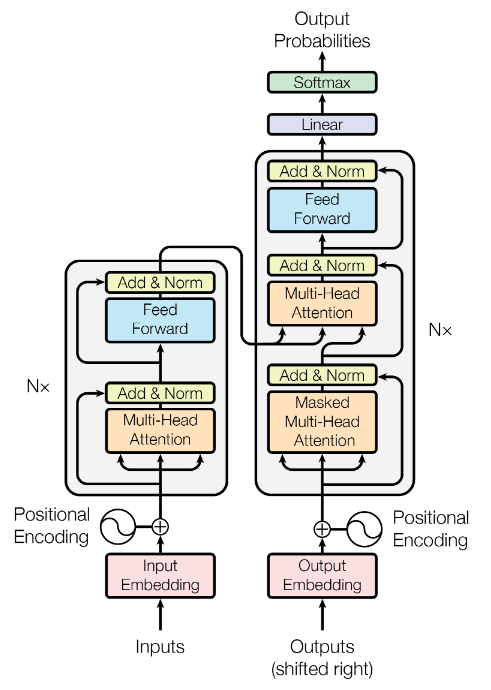
\includegraphics[width=0.55\linewidth]{figures/original_transformer_archi.png}
	\caption{Original Transformers architecture~\autocite{vaswaniAttentionAllYou}, akin to the previous example the encoder stack
		is situated on the left whilst the decoder is situated on the right.}
	\label{fig:transformer_architecture}
\end{figure}
\begin{itemize}
	\item \textbf{Black Arrows}: In~\Cref{fig:transformer_architecture}, the black arrows depict the dataflow.
	\item \textbf{Input Embeddings}: As can be seen at the bottom of the~\Cref{fig:transformer_architecture}, the \code{Inputs} are fed in to the encoder side and creates the
	      \code{Input Embedding}. \code{Outputs} flow into the decoder side and create the \code{Output Embedding}. This is only during inference. In training
	      the model works differently as the output is known and as such that known sequence is fed in to the decoder side. Part of the output embedding
	      is masked during training so the model doesn't `peek ahead'.
	      \bigbreak
	      In the original transformer architecture the input embeddings are a vector of a fixed size (this usually varies from model to model).
	      The input vectors combine the input sequence, actually a `tokenized' sequence (see \Cref{sec:tokenisation}) combined with the positional data
	      (1-D) of that particular token in the input sequence.
	\item \textbf{Add \& Norm}: The \code{Add \& Norm} refer to the addition of weights and a normalisation function, which uses `layer normalization'~\autocite{vijayraniaDifferentNormalizationLayers2021} to normalise.
	\item \textbf{Multi-Head Attention}: The \code{Multi-Head Attention} is the heart of the transformer. It is essentially numerous self attention layers stacked together (more
	      detail to follow).
	\item\textbf{Linear}: There are two linear translations in the \code{Linear} component which directly proceed a softmax function.
	\item \textbf{Feed Forward}: The feed forward neural network is a stack of layers. An input layer, some hidden layers and an output layer.
	      The data never flows backwards (back propagation) only forwards. The goal of the feed forward network is to approximate some function of the input.
	      \begin{figure}[H]
		      \centering
		      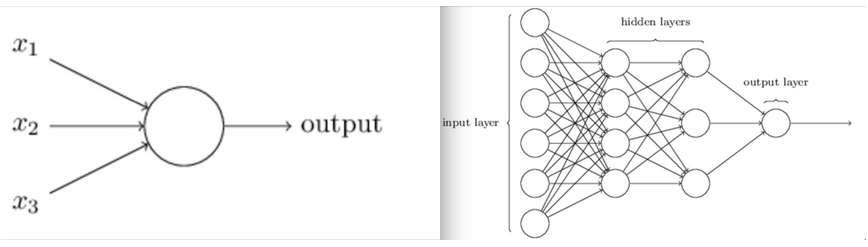
\includegraphics[width=1\linewidth]{figures/feed_forward.png}
		      \label{fig:feed_forward}
		      \caption{Classic Feed Forward Neural network layer architecture~\autocite{guptaDeepLearningFeedforward2018}, The left side depicts
			      a single perceptron whilst the right depicts a Multi-Layer Perceptron network.}
	      \end{figure}
	      They are also known as a \emph{Multi-Layer Perceptron (MLP)}. One of the first and most popular deep learning models~\autocite{FeedforwardNeuralNetwork2022}.
	\item \textbf{Softmax}: The Softmax function is used to compress the outputs to form a number in the range 0 - 1 \code{Output Probabilities}.
	\item Output Probabilities determine the token for that position. The token sequence is then sent back around to the start of the decoder stack.
	\item They are shifted right by one position as a special kind of token to indicate the start of a sequence.
	\item The process is repeated until the end of the sequence is reached - for inference, or until the epochs are completed - for training.
\end{itemize}

\subsection{Context}
\label{sec:context}
Human languages are a beautiful construct. The ability to express complex ideas and meanings to each other is fundamental
to our species evolution, both technical and cultural. But they are also incredibly complex to learn. There are many different syntaxes, rules and
of course, rule breakers. A word can take on a range of different meanings depending on the context (a homonym). \\
For example:
\begin{enumerate}
	\item \emph{The sound of a dog bark startled the cat.}
	\item \emph{The cat scampered up the tree bark.}
\end{enumerate}
The word \emph{bark} has two different meanings depending on the context. Humans are quite good at being able to tell which meaning
should be derived from the context, but trying to teach this to a machine is a much more complex task.
\bigbreak
This idea of context in a sentence as above can be thought of as the different geographical location of text blocks on a document,
in particular an invoice. To be able to extract the relevant meaning, the context is vital. As aforementioned, invoices
have no set standard and can vary significantly. During the creation of the dataset for this project an invoice was discovered
with two varying styles of expression for two vary similar products. It is one of three to four test emails used during system
development. A brief look through other documents corroborated that this type of finding is quite common across a multitude of
different suppliers invoices. This is an unfortunate trend.
\bigbreak
Both highlighted rows are identical in every field, except for the description.\\
The beers are even made by the same company, yet the description of the quantity was, presumably, left to be filled in by two different humans with
no structure or naming standards. With such inconsistencies in the data, the task of learning becomes more difficult and the concept of context
becomes extremely important.
\begin{figure}[H]
	\centering
	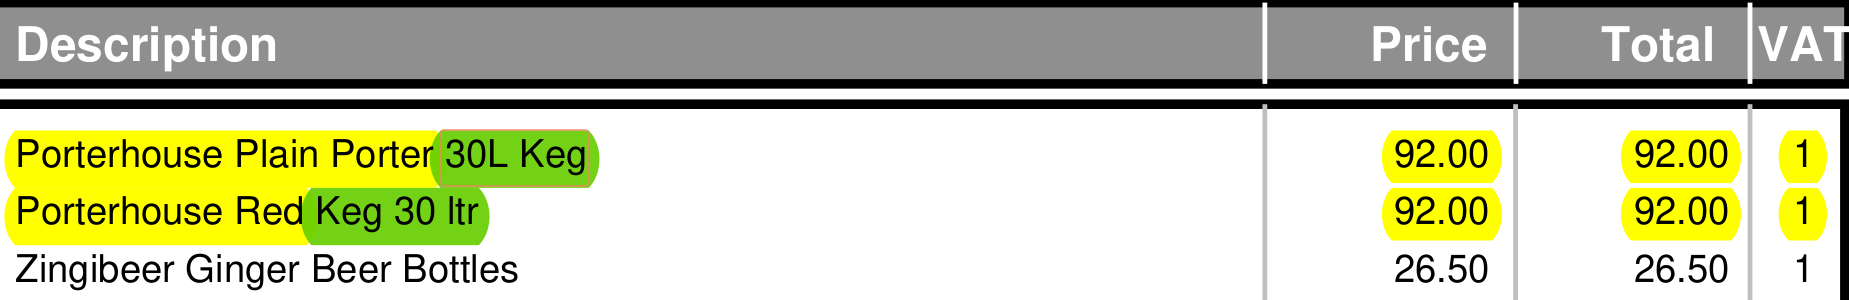
\includegraphics[width=1\linewidth]{figures/invo_complexity.png}
	\caption[Invoice depicting inconsistencies]{This is a real invoice depicting inconsistencies in the description, highlighted in green.}
	\label{fig:context}
\end{figure}
For optimal performance, a model would need to have a way of associating different parts of an invoice with similar parts of other invoices,
throughout different layouts to establish a pattern. The model would need to pay particular attention to the context of the data.
\bigbreak
To overcome the complexities of the human language, some pre-processing must first be performed on the text data to convert it to
numbers which the model can use to manipulate and ultimately learn from. The way that transformers based models remember the
distances between words, in sentences or what their \emph{closeness} / association is to other words by using the attention mechanism.
\bigbreak
To understand what that is, it is helpful to understand the data which flows into the model as the input. We have already
briefly touched on the \code{embedding} procedure for the original transformer model, but now we will look at it in more detail
as we compare it to LayoutLMv2. Possessing the knowledge of what data is in the input embeddings (and output embeddings) will allow us to
understand what the attention mechanism is doing.
\bigbreak
The main text model input string is not a sequence of words, but a sequence of \emph{tokens}.
\subsection{Tokenisation}
\label{sec:tokenisation}
To improve performance a body of text is first tokenized, or split into smaller chunks.\\
Tokenization usually comes in three different forms; there are word, subword and character-based tokenization methods \autocite{WhatTokenizationTokenization2020}.
\begin{itemize}
	\item \textbf{Word Tokenization}: A word is defined as a sequence of characters which are separated by a delimiter, usually, separated by a space.
	      This method has some drawbacks, like when the model encounters \emph{Out of Vocabulary words (OOV)}, these are words that the model has not encountered
	      in training and as such do not appear in the vocabulary.\\ There are some ways to deal with OOV words, but they are not very performative.
	      \bigbreak
	      A further issue is the size of the vocabulary. Pre-trained models, such as the transformers based models, are usually trained on a massive corpus of
	      data. As each unique encountered word is stored, the model size quickly explodes.
	\item \textbf{Character-Based Tokenisation}: A character-based tokenization is a method of tokenizing a text document by splitting the text into
	      individual characters. \\
	      The downside of character-based tokenization is that the model is not able to learn the meaning of the words as there are far more combinations of
	      individual characters than that of words. So detecting a pattern between these characters is extremely difficult. The vocabulary size is only
	      26.
	\item \textbf{Subword Tokenization}: A subword tokenization is a method of tokenizing a text document by splitting the text into subwords.
	      For example, the word \emph{smartest} is split into \emph{smart} and \emph{est}, whilst the word \emph{largest} is split into \emph{large} and \emph{st}.
	      The subword tokenization method is very performative, as it is able to learn the meaning of the words. If the model encounters an OOV word, it
	      will break it down and may learn meaning from the subwords and the subwords proximity to and from other words. \\
	      It is important to note that
	      this method will not split every word into subwords. Frequently occurring words are kept as is, whilst words that occurr less frequently
	      are split. This is highly dependent on the corpus, but as an example, the word \emph{annoy} will not be split, if the word \emph{annoying}
	      occurs frequently in the corpus then \emph{annoying} will also be kept. If however, it is rare in the corpus then it will be split
	      into \emph{annoy} and \emph{ing}. If they model encounters an OOV word such as \emph{annoyingly}. It can make sense of the word by splitting it
	      into \emph{annoy}, \emph{ing} and \emph{ly} then it will find subwords which match.
	      \bigbreak
	      There are many subword tokenization methods, but two shall be explained for relevance.
	      \begin{itemize}
		      \item \textbf{Byte-Pair Encoding (BPE)}: is a popular and performative method that initializes the vocabulary to include
		            every character present in the corpus, and each set of characters' (words) frequency is determined.
		            BPE then counts the frequency of each possible symbol pair that occurs most frequently and merges
		            them together. This merge strategy is repeated until stopped by the user. It is a tunable hyperparameter.\\
		            This is easier explained by looking at an example, as per the Hugging Face documentation~\autocite{SummaryTokenizers}:
		            \bigbreak
		            This is the corpus and frequency:\\
		            \code{("hug", 10), ("pug", 5), ("pun", 12), ("bun", 4), ("hugs", 5)}\\
		            Which gives us this base vocabulary:\\
		            \code{["b", "g", "h", "n", "p", "s", "u"]}\\
		            The first symbol pair chosen is: \\
		            \code{("u" + "g")}\\
		            As this combination appears most 10 + 5 + 5 = 20.\\
		            The symbol pair is added to the vocabulary: \\
		            \code{["b", "g", "h", "n", "p", "s", "u", "ug"]}
		            \bigbreak
		            The merging process is repeated until the user defined limit of the vocabulary size or number of merges is reached.
		      \item \textbf{WordPiece Tokenization}: is a subword tokenization method which is used in the LayoutLMv2 model. It is based on and is very similar to
		            the BPE method. The difference is that the BPE method chooses the most frequent symbol pair, whilst the WordPiece method uses probabilities.\\
		            As per our example:\\
		            \code{"u"} followed by \code{"g"} would only have merged if the probability of \code{"ug"} divided by \code{"u"}, \code{"g"} was greater
		            than any other pair.
	      \end{itemize}
\end{itemize}
Most of the Transformers architecture based models use some BPE or some variation of it.
\subsection{Multi Modal Token Embeddings}
These tokens are given numerical IDs which are kept in a look-up table.\\
The tokens are not the only data fed into the model. The \emph{multi-modality} refers to a combination of other data types. With the original
transformers architecture the 1-D position or position in a sequence is combined with the original input token. In the case of
LayoutLMv2, the multi-modality is the combination of the token and the position the initial training phase.
This is known as the \emph{Layout Embedding} and refers to the geometrical position of the token in the document.
As this is a requirement and a large part of the reason that this model is so performative, a list of bounding boxes must be provided to the model
upon calling it for training or inference. \\
The tokenizer process determines the bounding box (from the initial OCR'd input bounding boxes for words) per token in the tokenization stage.
\bigbreak
Furthermore, the segment embeddings are used to distinguish different text segments.\\
A further addition to the LayoutLMv2 model which again differs from the original transformers model is further input into the final embedding which
will traverse the system. This input is a visual representation AKA an \emph{image embedding} of the token~\autocite{LayoutLMExplained2022}.
As the document in JPG or PNG format is also passed in as a parameter when calling the model, the model is able to slice out the token locations
from the document. This is achieved in parallel to the token and position encoding via a \emph{Faster R-CNN}~\autocite{FasterRCNNExplained2020}.
LayoutMLv2 (the Hugging Face version) uses Detectron2~\autocite{FacebookresearchDetectron22022} as the Faster R-CNN which essentially acts as the model's visual backbone and
object detection algorithm.
\bigbreak
The combination of tokens, positional data in both the 1-D sequence and 2-D the entire document along with the visual aspect provided by the
Detectron2 and the segment embeddings are the final embedded input matrices. As detailed, these models are known as multi-modal as there are a variety of input mediums that constitute the
embeddings.\\
It is important to note that embedding only occurs once, in the initial input stage of the model.
\subsection{LayoutLMv2 Architecture}
Know having a greater understanding of the input for the LayoutLMv2 model we observe the architecture\footnote{The difference between the original LayoutLM and LayoutLMv2
	is that the visual and positional embedding occurs only during the fine-tuning phase for the original LayoutLM, whereas, LayoutLMv2 includes this
	data during the initial training phase too.}.
\begin{figure}[H]
	\centering
	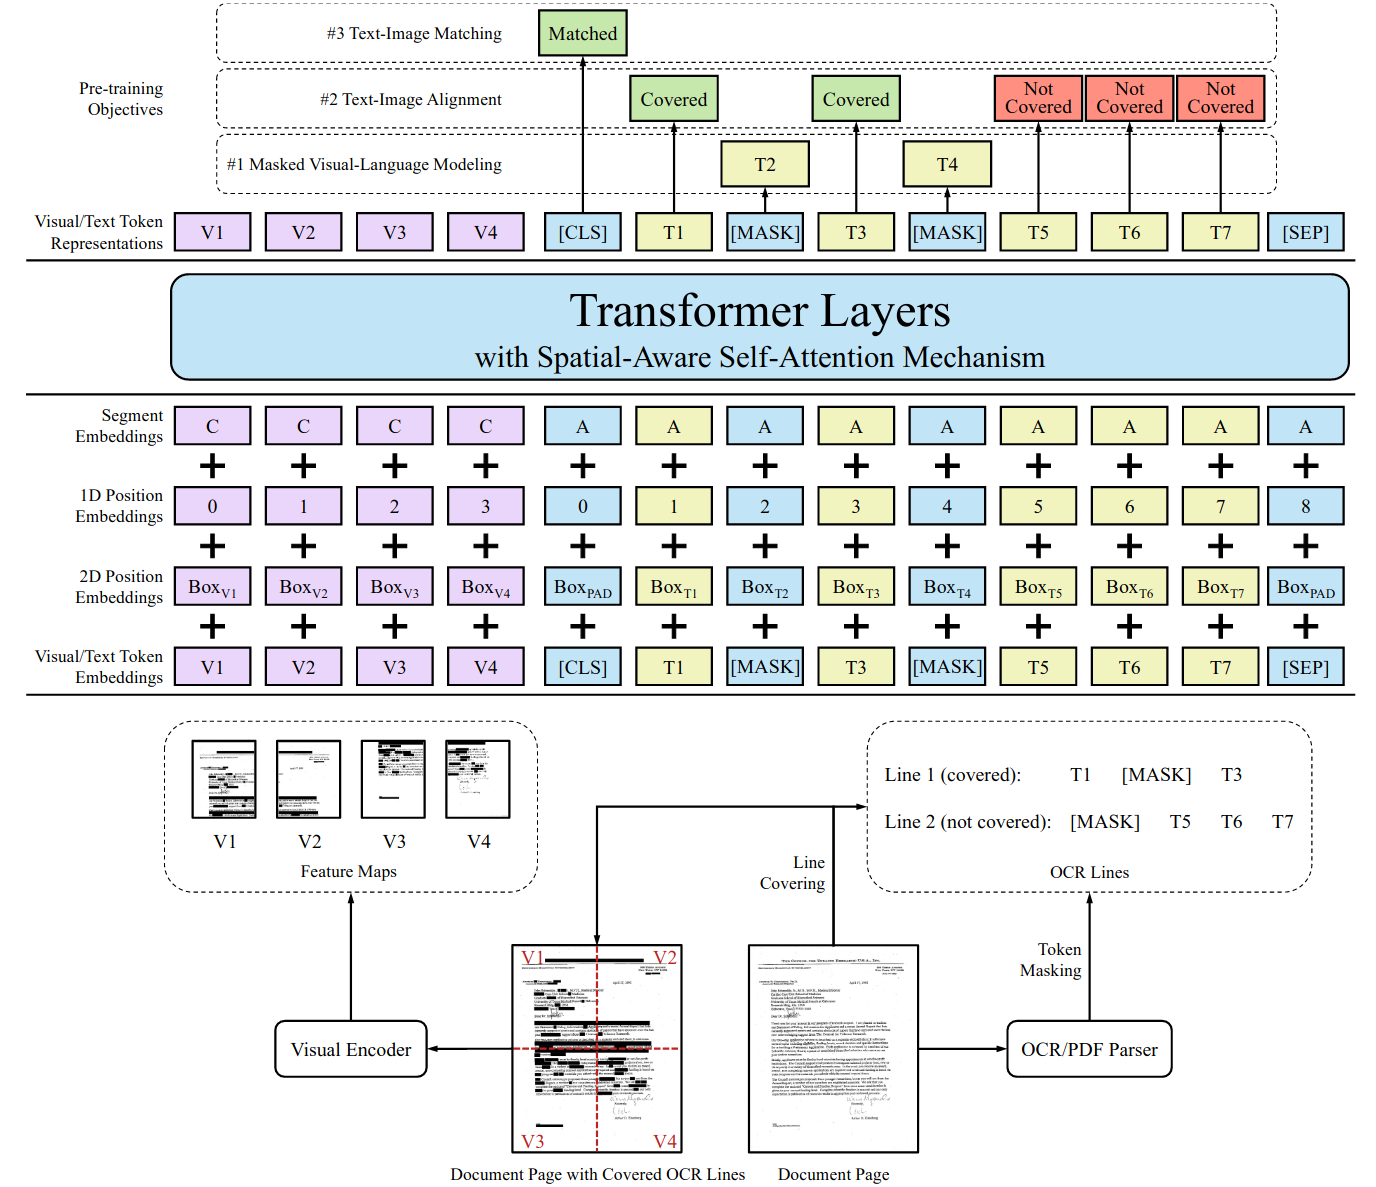
\includegraphics[width=1\textwidth]{figures/layoutlmv2_archi.png}
	\caption{LayoutLMv2 Architecture as per~\autocite{xuLayoutLMv2MultimodalPretraining2022}}
	\label{fig:layoutlmv2_archi}
\end{figure}

\#\# Should I swap the architecture image and the multi modal token embeddings section? it essentially explains the
layers, I kind of wanted to let the reader build an image in their head by reading it and then seeing the architecture.
That way it feels like the reader has been able to visualize / `come up with' the  architecture on their own.
I may not have done a good enough job in my descriptions though or maybe its just easer to map a diagram to a bullet list?
oh yea I should restructure that as a bullet list
\#\#
Observing \Cref{fig:layoutlmv2_archi}, it is useful to define some special case tokens which have not been covered thus far:
\begin{itemize}
	\item \textbf{[BOS]}: Beginning of sentence.
	\item \textbf{[EOS]}: End of sentence.
	\item \textbf{[UNK]}: Out-of-vocabulary tokens
	\item \textbf{[PAD]}: When a sequence size is smaller than expected constant sequence size padding is added. The model
	      knows to ignore the padding during processing due to its special type.
	\item \textbf{[CLS]}: to initialize the sequence.
	\item \textbf{[MASK]}: to mask tokens (for pre-training purposes).
\end{itemize}
Having already covered the basic transformer layers architecture, our attention can turn to the self attention mechanism.
\subsection{Multi-head Self Attention, Is All You Need}
Attention is they key component of the transformer architecture\footnote{Attention is also one of the more difficult concepts to grasp. These resources
	played a pivotal role in acquiring an understanding~\autocite{doshiTransformersExplainedVisually2021b}, here~\autocite{doshiTransformersExplainedVisually2021a},
	here~\autocite{cristinaTransformerAttentionMechanism2021}.
	and here~\autocite{alammarIllustratedTransformer}.}.
Remember the difficulties surrounding human language context?~(\Cref{sec:context}) This is the layer that attempts to capture and learn
the complexities of that context. Attention is used in the model in three places as per \Cref{fig:attention_usage}:
\begin{figure}[H]
	\centering
	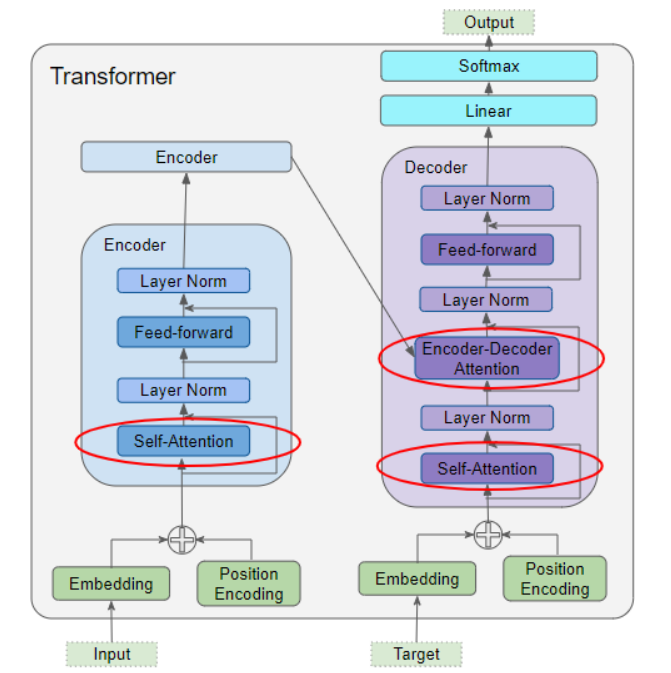
\includegraphics[width=0.7\textwidth]{figures/attention_usage.png}
	\caption[Attention Usage]{Attention is used in three places from here~\autocite{doshiTransformersExplainedVisually2021a}}
	\label{fig:attention_usage}
\end{figure}
\begin{itemize}
	\item Self-Attention in the Encoder.
	\item Self-Attention in the Decoder.
	\item Self-Attention in the Encoder-Decoder, also in the Decoder.
\end{itemize}
The attention layer has three input parameters namely, the \emph{Query (Q), Key (K), Value (V)}. All three of these parameters
are matrices of the same size.\\
From the input sequence every single word (actually embedding, but it is easier to think of it as a word and will be referred to as such in this section)
in the sequence is represented as a vector. In practice, this would be just like a single self-attention layer. As a Multi-head attention layer is used in this
model architecture this would be analogous to concatenating other word vectors to create a matrix. This is the difference between a regular self attention layer
and a multi-head attention layer, the increase in dimensionality. This increase in dimensionality brings with it many performance improvements, the model
can train and infer quicker. Along with more accurate results, higher dimensionalities allow for more details and relationships to be recorded.\\
For the sake of clarity this report will initially reduce the dimensionality and describe a single word vector.\\
This gives a matrix of size (Sequence Length, Embedding Size, \sout{Sample Size}) - as we have reduced dimensionality.
\bigbreak
The first step is to create a Query, Key and a Value matrix for each word in the input sequence. They are updated via the three separate linear layers
as per \Cref{fig:kvq_ll}. Each linear layer has its own weights~\autocite{alammarIllustratedTransformer}.
\begin{figure}[H]
	\centering
	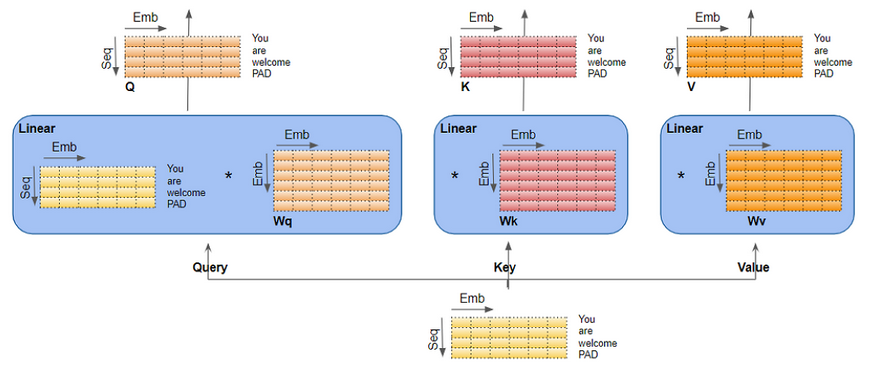
\includegraphics[width=1\textwidth]{figures/k_v_q_linear_layers.png}
	\caption{Key, Value and Query linear layers from here~\autocite{doshiTransformersExplainedVisually2021a}.}
	\label{fig:kvq_ll}
\end{figure}
In training the values for the linear layers are initially set randomly and are updated during training to return the
final weights\footnote{This depends on the training, pre-training or fine-tuning, these concepts will be covered in detail later.}. \\
For the multi-head attention layer the matrices are \textbf{logically} split up and distributed across the heads to allow for computation in parallel.
Choosing a \emph{query size} parameter determines the size of the logical partitioning.
\bigbreak
The important part to note here is that each input word has gone through a series of transformations. Position encoding, Embedding and the Linear
Layers.\\
Each of these translations is tunable, and it is how the model learns. When a predicted output is wrong, the weights are altered to reflect the
wrong decision. Similarly, for correct output in the training phase, the weights are altered to reflect the correct decision.
\subsection{Attention Score}
First this report will tackle the attention in the encoder. The attention used in the decoder is very similar to the attention in the encoder. \\
This is the formula used to calculate the attention score.
\begin{figure}[H]
	\centering
	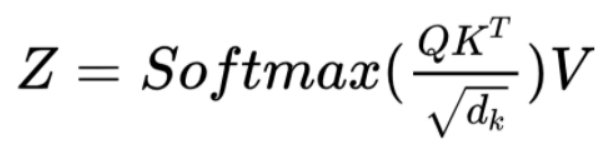
\includegraphics[width=0.7\textwidth]{figures/attention_score_formula.png}
	\caption{Attention Score Formula}
	\label{fig:attention_score}
\end{figure}
Where:
\begin{itemize}
	\item \textbf{Q} is the query matrix.
	\item \textbf{K} is the key matrix.
	\item \textbf{V} is the value matrix.
	\item \textbf{QK\textsuperscript{T}} is the dot product of the query matrix and the transpose of the key matrix.
	\item \textbf{d\textsubscript{k}} is the dimensionality of the key matrix.
\end{itemize}
A nice way to visualise this can be seen in the figure~\cref{fig:attention_score_matrix_form}.
\begin{figure}[H]
	\centering
	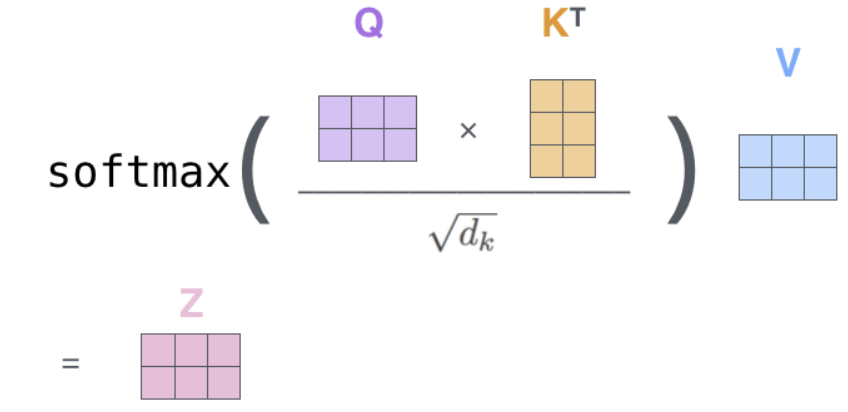
\includegraphics[width=0.7\textwidth]{figures/attention_formula_matrix_form.png}
	\caption{Attention Score Formula visualized in the context of matrices. From this source~\autocite{alammarIllustratedTransformer}}
	\label{fig:attention_score_matrix_form}
\end{figure}
The attention layer itself can be visualized in the figure~\cref{fig:attention_layer}.
\begin{figure}[H]
	\centering
	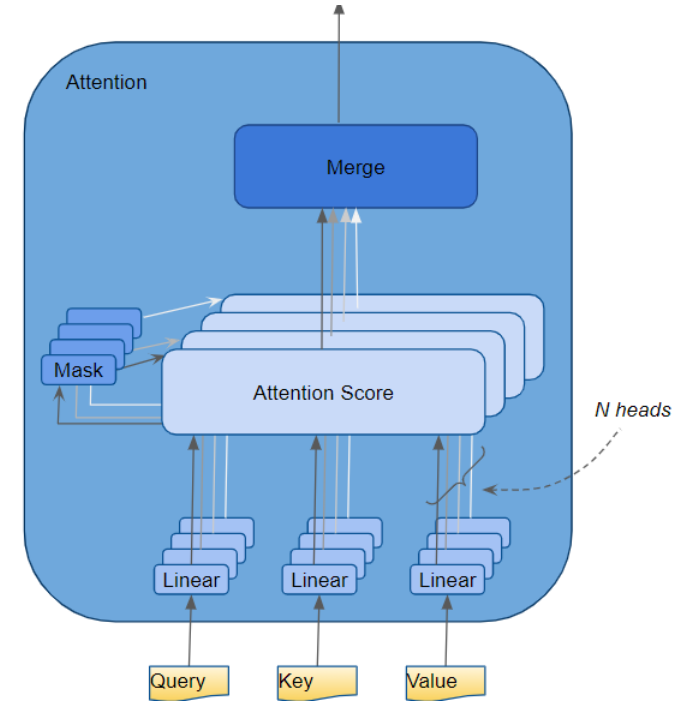
\includegraphics[width=0.6\textwidth]{figures/attention_layer.png}
	\caption{Attention Layer in detail from here~\autocite{doshiTransformersExplainedVisually2021b}.}
	\label{fig:attention_layer}
\end{figure}
As the multi-headed attention is logically partitioned, separate weight matrices are used for each head. As can be visualised in the
\cref{fig:attention_layer_heads}. In this example, the words `Thinking Machines' form the input matrix (a vector for each word)\footnote{
	In the use case for invoices, the input matrix X consists of the final embeddings, as derived earlier.}.
\begin{figure}[H]
	\centering
	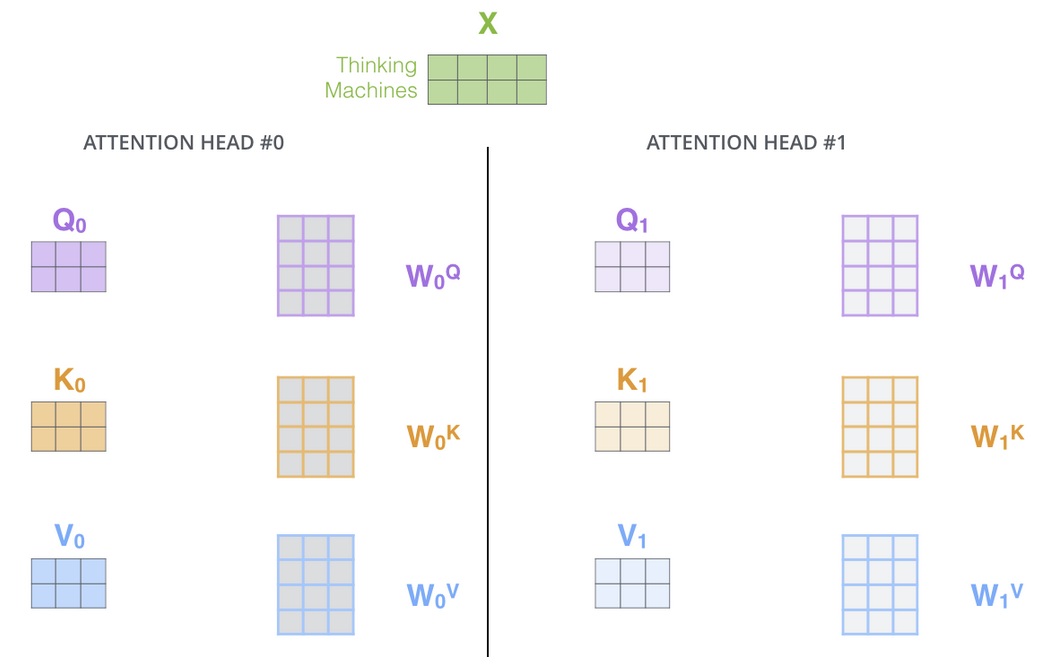
\includegraphics[width=0.9\textwidth]{figures/attention_multi_head.png}
	\caption{Attention Layer with heads from here~\autocite{alammarIllustratedTransformer}}
	\label{fig:attention_layer_heads}
\end{figure}
After the self attention scores have been calculated (\Cref{fig:attention_score_matrix_form}) for each attention head as there are now
eight separate matrices (one for each attention head\footnote{Eight is the default value, although this can be configured.}). The correct shape
must be obtained to satisfy the desired input shape of the feed forward layer. This layer is expecting a single matrix, so the attention heads
the matrices are simply concatenated and multiplied with a further weight matrix obtained\footnote{This weight matrix is adjusted during training.} as per
\Cref{fig:concat_atn_head_matrices}. The idea here is to keep the values of the words that are relevant and drown out the irrelevant words by multiplying
them by tiny numbers, i.e. 0.01. This returns the desired effect.
\begin{figure}[H]
	\centering
	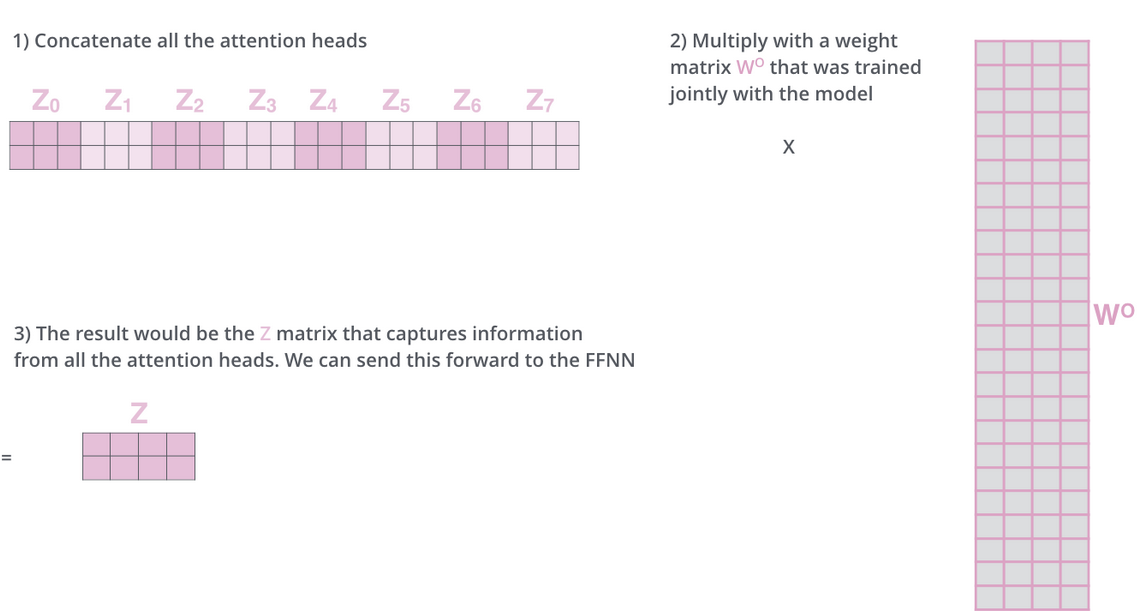
\includegraphics[width=0.9\textwidth]{figures/concat_atn_head_matrices.png}
	\caption{Concatenated Attention Head Matrices as sourced from here~\autocite{alammarIllustratedTransformer}}
	\label{fig:concat_atn_head_matrices}
\end{figure}
\Cref{fig:atn_summary} depicts a way to visualze the entire process. As previously detailed, and can be seen, the embeddings are only
used in the inital pass into the encoder, all subsequent traversals use \code{R}, which is the output of the encoder directly preceding the
current encoder.
\begin{figure}[H]
	\centering
	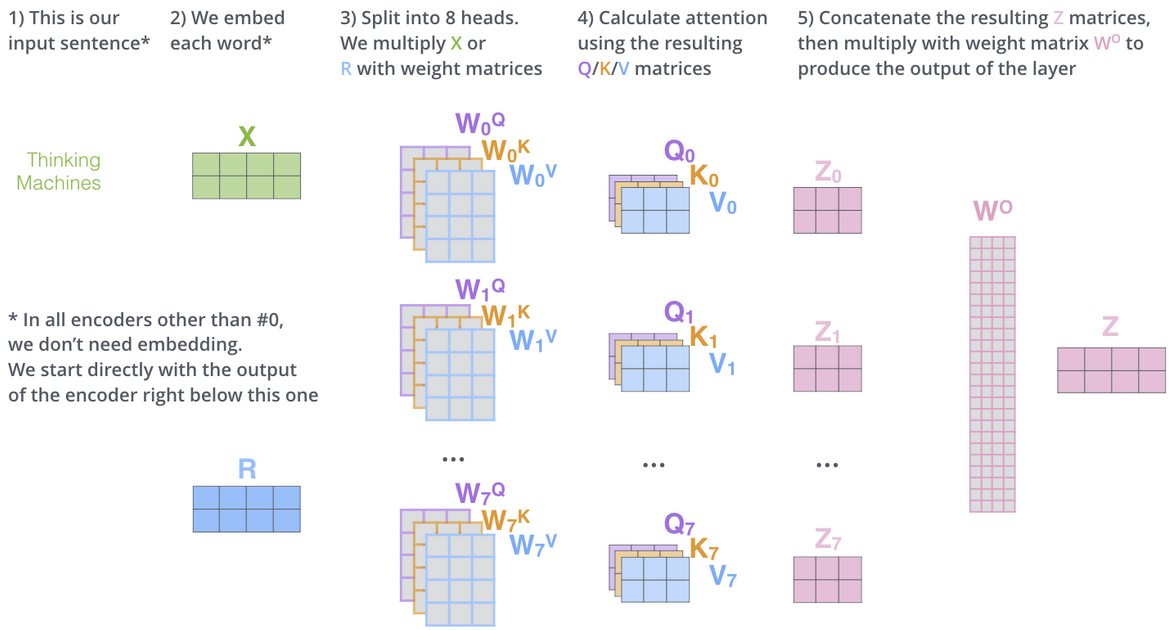
\includegraphics[width=1\textwidth]{figures/atn_summary.png}
	\caption{Attention Summary from here~\autocite{alammarIllustratedTransformer}}
	\label{fig:atn_summary}
\end{figure}
The attention score calculation is carried out in step \textbf{4} as depicted in \Cref{fig:atn_summary}. \\
\subsection{Attention Intuition}
The formula along with its place in the encoder and the inputs have now been detailed, yet it is important to develop an intuition of
why the formula works and how this formula returns useful scores.\\
To do this here is an example starting with the dot product calculation of the Query (Q) and Key (K)\textsuperscript{Transpose} matrices
as per the formula and depicted in \Cref{fig:q_kt_dot_product}. Lets call this the `factor matrix'.
\begin{figure}[H]
	\centering
	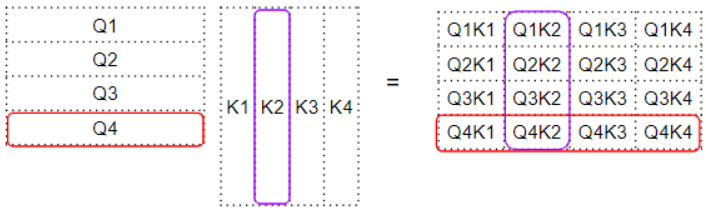
\includegraphics[width=0.7\textwidth]{figures/dot_prodct_q_kt.png}
	\caption{Dot Product of Query and Key Transpose sourced from here~\autocite{doshiTransformersExplainedVisually2021b}}
	\label{fig:q_kt_dot_product}
\end{figure}
Other calculations the division and square root of the formula are not shown here, as they do not alter the matrix but merely configure its
shape and manipulate it so that the score can be calculated more easily.
\bigbreak
Now that the dot product of (QK\textsuperscript{T}), the next part of the formula is to obtain the
dot product of the result of (QK\textsuperscript{T})\footnote{Query Key\textsuperscript{T}} with the V or Values matrix as per \Cref{fig:qk_v_dot_product}.
\begin{figure}[H]
	\centering
	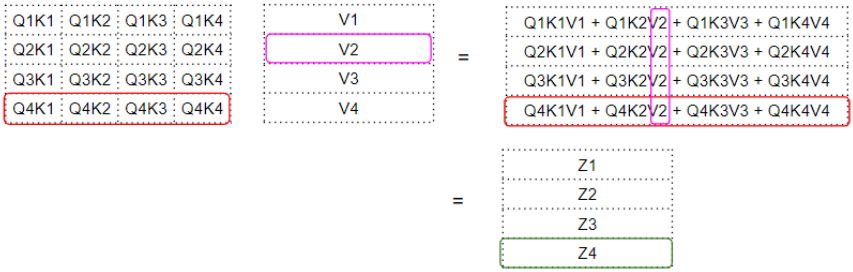
\includegraphics[width=1\textwidth]{figures/qk_v_dot_product.png}
	\caption{Dot Product of Query Key Transpose and Values sourced from here~\autocite{doshiTransformersExplainedVisually2021b}, depicting the
		resulting attention score.}
	\label{fig:qk_v_dot_product}
\end{figure}
Z is the resulting attention score vector. A way to understand the sequence of events is to think about the ouput score.
For each word, the attention score is the encoded value of every word from the `Value' matrix, weighted by the `factor'
matrix. The factor matrix itself is the dot product of the Query value for the specified word with the Key value of all
words as\autocite{doshiTransformersExplainedVisually2021b} per \Cref{fig:atn_weight_summation}.
\begin{figure}[H]
	\centering
	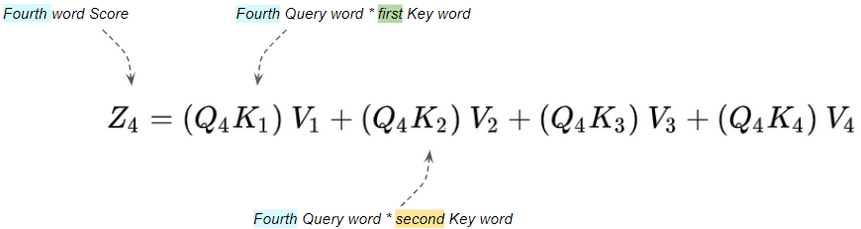
\includegraphics[width=0.9\textwidth]{figures/atn_weight_summation.png}
	\caption{Attention Weight Summation from here~\autocite{doshiTransformersExplainedVisually2021b}, depicting the resulting attention score.}
	\label{fig:atn_weight_summation}
\end{figure}
Here the Query word is the word for which the attention is being calculated, the Key and Value word is the word to which we
are paying attention to determine how relevant that word is to the Query word\autocite~{doshiTransformersExplainedVisually2021b}.
\bigbreak
Remember that the Query, Key and Value rows are actually vector projections of the words with their added embeddings i.e. positional attributes etc.,
then as the dot product between a particular word and every other word captures some interactions between the word and all others, this
ability is utilized to signify the relationship or proximity of any word with any word. \\
A little visual aid may be beneficial, \Cref{fig:dot_prod_similarity}:
\begin{figure}[H]
	\centering
	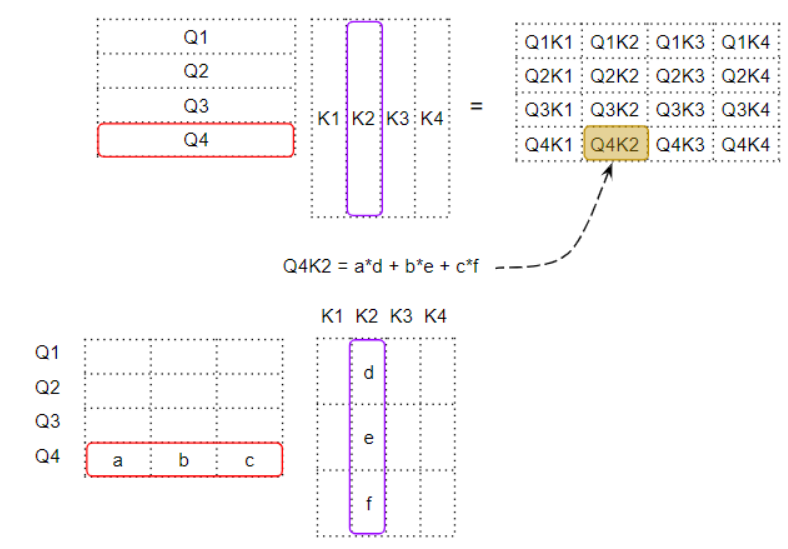
\includegraphics[width=0.9\textwidth]{figures/dot_prod_similarity.png}
	\caption{Dot Product of Query, Key and Value from here~\autocite{doshiTransformersExplainedVisually2021b}, depicting the resulting attention score.}
	\label{fig:dot_prod_similarity}
\end{figure}
This is excellently explained here~\autocite{doshiTransformersExplainedVisually2021b}:
\begin{itemize}
	\item If any two paired numbers, like `a' and `d'', are both positive or both negative then the product wil be positive. The product will
	      increase the summation.
	\item If one number is positive but the other negative then teh product will be negative. The product will decrease the summation.
	\item If the product is positive, the larger both numbers are, the more they contribute to the summation.
\end{itemize}
If the signs of the corresponding numbers in the two vectors are aligned, the final sum will be larger. This means a higher level of similarity,
or proximity between the two words.\\
For word vectors that are aligned the attention score is high, and vice versa for word vectors which are not aligned.
The ability to tune the parameter of the translations during training gives the model the ability to strengthen or weaken the alignment of the
words.
\bigbreak
As can be seen in \Cref{fig:attention_usage}, attention is used in three areas. The main concept and how attention works in the encoder has
been detailed. The other two areas are as follows.
\subsection{Self Attention in the Decoder}
The self attention mechanism in the decoder works in a similar fashion to the encoder, but the inputs are different as per \Cref{fig:atn_decoder}.
\begin{figure}[H]
	\centering
	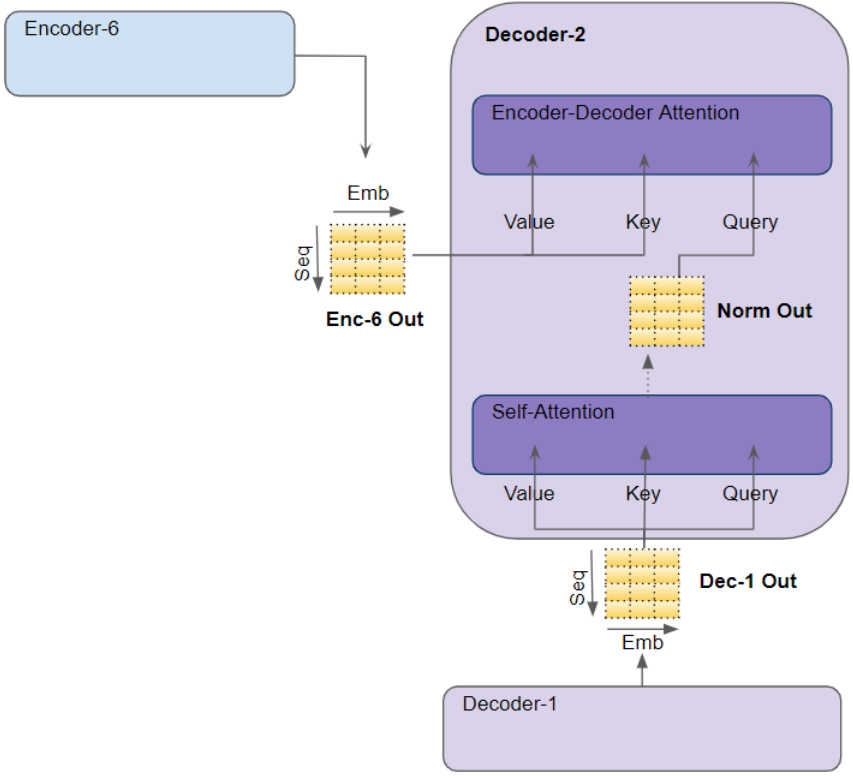
\includegraphics[width=0.8\textwidth]{figures/atn_decoder.png}
	\caption{Self Attention Mechanism for Decoder from here~\autocite{doshiTransformersExplainedVisually2021b}, depicting the resulting attention score.}
	\label{fig:atn_decoder}
\end{figure}
In the decoder the relevance of each word in the target sentence is computed with respect to every other word in the target sentence
as per \Cref{fig:decoder_self_atn}.
\begin{figure}[H]
	\centering
	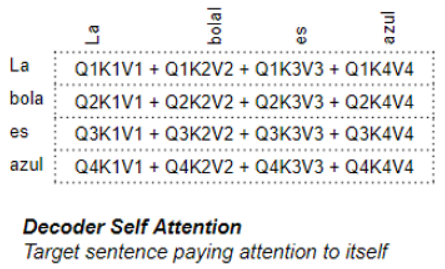
\includegraphics[width=0.6\textwidth]{figures/decoder_self_atn.png}
	\caption{Attention Mechanism for Encoder-Decoder in the decoder from here~\autocite{doshiTransformersExplainedVisually2021b}.}
	\label{fig:decoder_self_atn}
\end{figure}
\subsection{Attention in the Encoder-Decoder}
Again, very similar to the encoder attention but the Query is obtained from the target sentence and the Key and Value are obtained from the
source sentence. The goal is to compute the relevance of each word in the target sentence to each word in the source sentence.
\begin{figure}[H]
	\centering
	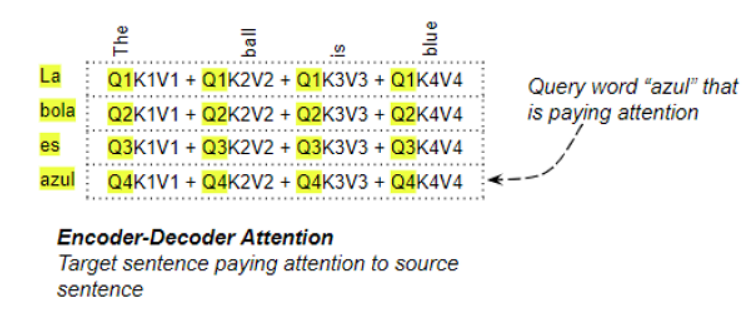
\includegraphics[width=0.9\textwidth]{figures/encoder_decoder_atn.png}
	\caption{Attention Mechanism for Encoder-Decoder from here~\autocite{doshiTransformersExplainedVisually2021b}. Same input
		and target as \Cref{fig:atn_decoder}.}
	\label{fig:atn_encoder_decoder}
\end{figure}
\subsection{Transfer Learning}
The architecture of the transformer allows for the model to be trained twice. \\
Transfer learning is a technique which allows a model to be trained on a dataset or numerous datasets to be used as its base corpus. The initial
training of these models requires huge amount of data and compute power along with expertise in the domain.
This is the base trained model.
\bigbreak
As an example, The \emph{BigScience Large Language Model}~\autocite{BigScienceResearchWorkshop}
is a model that is currently in training. The training of BigScience's main model started on March 11, 2022 11:42am PST and will continue
for 3-4 months on 384 A100 80GB GPUs of the \emph{Jean Zay} public supercomputer~\autocite{BigscienceTr11176BmllogsHugging}. The data set
contains 341.6 billion tokens. which is approx. 1.5 TB of data.\\ That is an astonishing amount of compute, data and engineering expertise.\\
This example is one of the more extreme but shows the scale of what the initial base training can be.
\bigbreak
In the case of LayoutLMv2, the base model has been trained on six different datasets, from the
visually-rich document understanding area including the aforementioned, SROIE dataset and others including the FUNSD dataset~\autocite{FUNSD}
and the CORD dataset~\autocite{CORDConsolidatedReceipt2022}.
\bigbreak
These models are then \emph{fine-tuned} on custom datasets for the specific task at hand. For example, LayoutLMv2 in this instance is
fine-tuned on the custom invoice dataset which is optimized for invoices but the same base model would also be used for receipts and other
documents which see a drastic shift in document layout. A model optimized for invoices may still work for some receipts, but to obtain
state-of-the-art results, the model should be fine-tuned on the dataset for which it will be used to infer.\\
A downstream task\footnote{A downstream task can be thought of as a models capabilities or different implementations, for example,
	LayoutLMv2 can be used for token classification (like this project) but it can also be used for \emph{Sequence Classification}
	and \emph{Question Answering} tasks~la\autocite{LayoutLMV2}.} to first classify what structure the document is and then use a trained model that is optimized for
that document structure could be implemented to further increase the accuracy of the system.
\bigbreak
This idea of transfer learning cuts out the large training time and allows most anyone to use and fine-tune a model to their specific needs.
Some libraries now exist which contain not only the pretrained models, but datasets of varying sizes and forms, along with other components
to aid in the pre-processing of the data to be used in the fine-tune training with model phase.\\
The \emph{transformers library} by Hugging Face~\autocite{HuggingFaceAI} is one such library.

\section{Hugging Face}
% stick that in a footnote
Hugging Face~\autocite{HuggingFaceAI} is a French company which initially developed a chat app that has since pivoted into becoming one of the most
popular deep learning model platforms~\autocite{syalHuggingFaceStep2020}. Here is what they say about themselves:
\begin{quoting} 
	Hugging Face Transformers provides APIs to easily download and train state-of-the-art pretrained models. Using pretrained models can reduce your compute
	costs, carbon footprint, and save you time from training a model from scratch. The models can be used across different modalities such as:
	text, audio, images, video, and multimodal.
	\begin{flushright}
	~---~Hugging Face Team
	\end{flushright}
\end{quoting}
They specialise in Natural Language Processing (NLP) and they have a large number of models available for public use.\\ 
The company provide the \code{Transformers} library which contains over thirty pre-trained models base models available
in over 100 languages~\autocite{HuggingFaceTransformers}. The models are mostly of based on the transformers architecture.\\
Hugging Face also provide \emph{The Model Hub}~\autocite{ModelsHuggingFace}, this works akin to a code repository for models, once a model is uploaded to the hub, it can be 
made public or private. Hugging Face also provide a large variety of open-source datasets~\autocite{HuggingFaceAIa} which can be used to train models.\\
The team have a massive amount of tutorials and guides on model architecture available along with a large number of articles, blogs and open-sourced code for 
model evaluation, training and inference.
\bigbreak
They make money via their Inference API where there are a plethora of models ready behind endpoints for a variety of different use cases. 
They also charge for support and for deployment and training of models on their servers.
\bigbreak
Transformers library is a very powerful library, it looks to cut away at the \emph{boiler-plate} code required to implement a model.\\
The library supports the PyTorch, TensorFlow and JAX frameworks. It even supports cross framework deployment so a model may be trained using 
PyTorch and deployed using TensorFlow or JAX for inference. All cross framework integrations appear to be supported~\autocite{Transformers}.\\
The library also contains some great functions for data pre-processing:
\begin{itemize}
	\item \textbf{Tokenizer}: The pre-processing step to convert text into a sequence of tokens.
	\item \textbf{FeatureExtractor}: This function resizes images for use in models and can even be used with the OCR engine enabled (PyTesseract).
	\item \textbf{Processor}: This is a model specific function which wraps the tokenizer and the feature extractor in to a single function for 
	ease of use.
\end{itemize}
The tokenizer is utilized in this project. \\
The transformers library along with the available resources on the Hugging Face website were used extensively during the research and development
phases of the project.
\subsection{}
use.


Before the Vaswani's et al. paper, \emph{Attention Is All You Need}, the state-of-the-art models for NLP were Recurrent Neural Networks
(RNNs) and Convolutional Neural Networks (CNNs) which implemented an encoder and a decoder
~\autocite{brownleeEncoderDecoderRecurrentNeural2017}. \\
The paper, along with subsequent varied implementations of it coupled with the utility of provisioning a model of such complexity, 
are responsible for a shift away from these models toward the transformer architecture.

\subsection{The Challenges}
\label{sec:challenges}
A kubernetes Ingress exposes HTTP and HTTPS traffic
from outside the cluster to services inside the cluster. Rules are defined in the Ingress resource and these rules control the
traffic
